\documentclass{beamer}
\usepackage[utf8]{inputenc}
\usepackage[english, russian]{babel}
\title{Представление графической информации. Булевы функции} 
\subtitle{Экзаменационный билет №7}
\author{Студент группы 8871 Ковлягин В.В.}
\usepackage{ragged2e}
\usepackage{booktabs}
\usepackage{tabularx}
\usepackage{tikz}
\usepackage{float}
\usepackage{graphicx}
\usetikzlibrary{calc, shapes, backgrounds}
\usepackage{amsmath, amssymb}
\usepackage{url} 
\usepackage{listings}
\frenchspacing
\begin{document}
\parindent=1cm
  \frame{\maketitle}
  \AtBeginSection[]{
    \begin{frame}<beamer>
      \tableofcontents[currentsection]
    \end{frame}}
    \section{Вопросы}
    \subsection{Представление графической информации}
    \begin{frame}{Представление графической информации}
        Создавать и хранить графические объекты в компьютере можно двумя способами: как растровое или как векторное изображение.
     Для каждого типа изображения используется свой способ кодирования.\\
   \\
     Растровое изображение представляет собой совокупность точек, используемых для его отображения на экране монитора.\\
    \\
     Объём растрового изображения определяется как произведение количества точек и информационного объёма одной точки, который зависит от количества возможных цветов. Для черно-белого изображения информационный объём одной точки равен  1  биту, так как точка может быть либо чёрной, либо белой, что можно закодировать одной из двух цифр —  0  или  1 .
    \end{frame}
\begin{figure}[H]
\begin{center}
\begin{minipage}[h]{0.65\linewidth}
\center{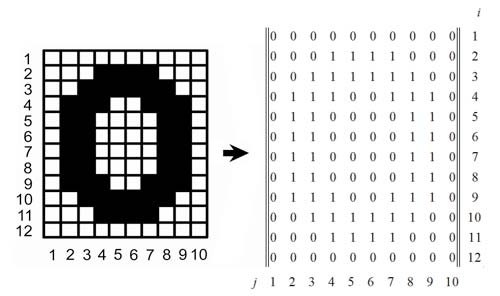
\includegraphics[width=1\linewidth]{rastr.png}}  \\
\frametitle{ Рис 1. Представление черно-белого растрового изображения в двоичной кодировке}
\end{minipage}
\end{center}
\end{figure}
Информационный объём растрового изображения (V) определяется как произведение числа входящих в изображение точек (N) на информационный объём одной точки (q), который зависит от количества возможных цветов, т.е. V=N⋅q\\

Если между чёрным и белым цветами имеется ещё шесть оттенков серого (всего  8), то информационный объём точки равен 3 бита (log28 = 3). Информационный объём такого изображения увеличивается в три раза:  V = 30000 бит.\\
 \newpage
Рассмотрим, сколько потребуется бит для отображения цветной точки: для  8  цветов необходимо  3  бита; для  16 цветов —  4  бита; для  256  цветов —  8  битов (1  байт). В таблице ниже представлено кодирование цветовой палитры из  16  цветов.\\
\begin{figure}[H]
\begin{center}
\begin{minipage}[h]{0.7\linewidth}
\center{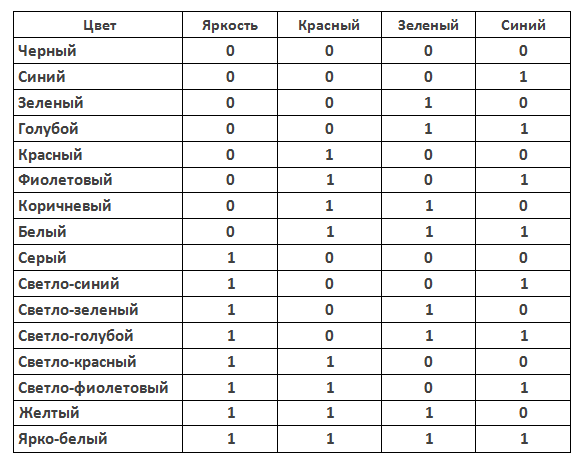
\includegraphics[width=1\linewidth]{palitra16.png}}  \\
\frametitle{ Рис 2. Таблица кодировки ячеек для различных цветов и оттенков}
\end{minipage}
\end{center}
\end{figure}
\newpage
\indentРазные цвета и их оттенки получаются за счёт наличия или отсутствия трёх основных цветов (красного, синего, зеленого) и степени их яркости. Каждая точка на экране кодируется с помощью  4  битов.\\
Цветные изображения могут отображаться в различных режимах, соответственно изменяется и информационный объём точки.
\begin{figure}[H]
\begin{center}
\begin{minipage}[h]{1\linewidth}
\center{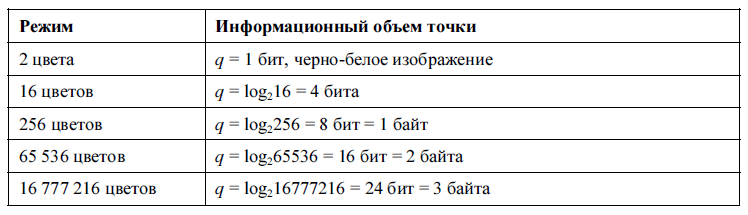
\includegraphics[width=1\linewidth]{rezhim.png}}  \\
\frametitle{ Рис 3. Цветовые режимы и соответствующие им объемы точек}
\end{minipage}
\end{center}
\end{figure}
Чем больше глубина цвета, тем больше объем графического файла.\\
\newpage
Векторное изображение представляет собой совокупность графических примитивов. Каждый примитив состоит из элементарных отрезков кривых, параметры которых (координаты узловых точек, радиус кривизны и пр.) описываются математическими формулами.\\
Информация о векторном рисунке кодируется обычным способом, как хранятся тексты, формулы, числа, т. е. хранится не графическое изображение, а только координаты и характеристики изображения его деталей. Поэтому для хранения векторных изображений требуется существенно меньше памяти, чем растровых изображений.\\
\newpage
    \subsection{Компрессия с потерей и без потери информации}
    \begin{frame}{Компрессия данных}
Сжатие данных с потерями — метод компрессии данных, при использовании которого распакованные данные отличаются от исходных, но степень отличия не существенна с точки зрения их дальнейшего использования.\\
В целом ряде случаев сжатие графики с потерями, обеспечивая очень высокие степени компрессии, практически незаметно для человека. Однако методы сжатия с потерями обладают и рядом недостатков:\\
Первый заключается в том, что компрессия с потерями применима не для всех случаев анализа графической информации. Например, фотография человеческого лица с незначительными изменениями в результате сжатия все еще остается пригодной для распространения в социальной сети, но применение "неточного" изображения при пересылке медицинских снимков негативно скажется на результатах анализа. Так же, изменения незаметные человеческому глазу могут повлиять на машинный метод анализа графической информации для машинного анализатора.\\
\begin{figure}[H]
\begin{center}
\begin{minipage}[h]{1\linewidth}
\center{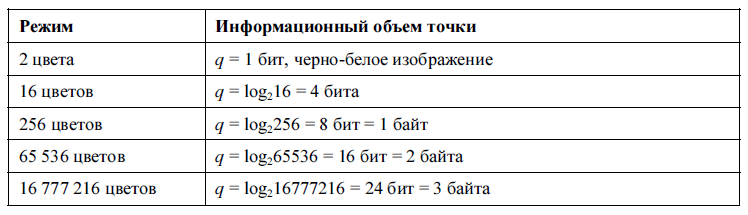
\includegraphics[width=1\linewidth]{rezhim.png}}  \\
\end{minipage}
\end{center}
\end{figure}
\end{frame}
Вторая причина заключается в том, что повторная компрессия и декомпрессия с потерями приводят к эффекту накопления погрешностей. Если говорить о степени применимости формата JPEG, то, очевидно, он полезен там, где важен большой коэффициент сжатия при сохранении исходной цветовой глубины. Именно это свойство обусловило широкое применение данного формата в представлении графической информации в Интернете, где скорость отображения файла имеет первостепенное значение.\\
Отрицательное свойство формата JPEG — ухудшение качества изображения, что делает практически невозможным его применение в полиграфии, где этот параметр является определяющим.\\
\newpage
\begin{frame}
Сжатие, или кодирование, без потерь может применяться для сжатия любой информации, поскольку обеспечивает абсолютно точное восстановление данных после кодирования и декодирования. Сжатие без потерь основано на простом принципе преобразования данных из одной группы символов в другую, более компактную.\\

Наиболее известны два алгоритма сжатия без потерь: это кодирование Хаффмена (Huffman) и LZW-кодирование (по начальным буквам имен создателей Lempel, Ziv, Welch), которые представляют основные подходы при сжатии информации. Кодирование Хаффмена появилось в начале 50-х; принцип его заключается в уменьшении количества битов, используемых для представления часто встречающихся символов и соответственно в увеличении количества битов, используемых для редко встречающихся символов. Метод LZW кодирует строки символов, анализируя входной поток для построения расширенного алфавита, основанного на строках, которые он обрабатывает.
\end{frame}


\subsection{Форматы BMP, GIF, JPEG}
\begin{frame}{Форматы BMP, GIF, JPEG}
Расширение BMP обычно используется для хранения растровых изображений. .BMP – это стандартный, не сжатый битовый графический формат, используемый в Windows. BMP файл хранить графику в формате, который называется аппаратно-независимый растр. Файл .BMP состоит из заголовка файла (растровый идентификатор, размер файла, ширина, высота, варианты цвета, и растровые данные начальной точки), заголовка изображения (может отсутствовать), палитры (может отсутствовать) и самого изображения.\\
\begin{figure}[H]
\begin{center}
\begin{minipage}[h]{0.25\linewidth}
\center{
\includegraphics[width=1\linewidth]{bmp-512.png}}  \\
\end{minipage}
\end{center}
\end{figure}
\end{frame}
\begin{frame}
GIF файл представляет из себя изображение, достаточно часто сопровождающееся анимацией. Формируется посредством специализированных графических редакторов, может нести в себе несколько растровых изображений в определенной последовательности. Формат GIF имеет распространение в сфере создания баннеров, а также графической оболочки видео-контента.\\
Основным преимуществом считается сжатие данных без явной потери качества при глубине до 256 цветов, современные редакции анимации GIF, включили в себя настраиваемые функции прозрачности. Анимированные изображения состоят из некоторого числа статичных кадров, а также данных о требуемом времени демонстрации того или иного кадра.\\
\begin{figure}[H]
\begin{center}
\begin{minipage}[h]{0.25\linewidth}
\center{
\includegraphics[width=1\linewidth]{no-translate-detected_318-45820.jpg}}  \\
\end{minipage}
\end{center}
\end{figure}
\end{frame}
\begin{frame}
Файлы с расширением JPEG удобны в случае необходимости отправки изображений по Интернету благодаря тому, что они сжимают такие изображения с определенной потерей качества. Формат JPEG предусматривает такой способ представления изображений, при котором сразу же после загрузки части изображения появляются размытые очертания всего файла (это отличает данный формат от форматов, которые предусматривают показ только загруженной части изображения). Степень сжатия можно регулировать, достигая при этом максимально выгодного соотношения размера файла и качества. Изображения JPEG также можно сохранять в формате JPG.\\
\begin{figure}[H]
\begin{center}
\begin{minipage}[h]{0.25\linewidth}
\center{
\includegraphics[width=1\linewidth]{jpeg-512.png}}  \\
\end{minipage}
\end{center}
\end{figure}
\end{frame}
    \subsection{Булевы функции, примеры, конъюнкция, дизъюнкция}
    \begin{frame}{Булевы функции}
Булева функция – это функция, аргументы и значение которой принадлежит множеству $\{0,1\}$. Булевы функции называются также функциями алгебры логики, двоичными функциями и переключательными функциями.\\
Булеву функцию от n переменных можно задать таблицей истинности, в которой наборы значений аргументов расположены в порядке возрастания их номеров: сначала идет набор, представляющий собой двоичное разложение 0 (этот набор имеет номер 0); затем идет набор, являющийся двоичным разложением 1, потом 2, 3 и т.д. Последний набор состоит из n единиц и является двоичным разложением числа 2^n -1 (такой порядок расположения наборов назовем лексикографическим порядком). Учитывая, что отсчет начинается с 0, а значение булевой функции может быть либо 0 либо 1, заключаем, что существует всего 2^(2^n) различных булевых функций от n переменных. Таким образом, имеется, например, 16 булевых функций от двух переменных, 256 — от трех и т. д.\\
    \end{frame}
Пример: Рассмотрим устройство, фиксирующее принятие решение тремя членами комиссии. Каждый член комиссии принимает решение нажимая на одну из двух кнопок.  Это фиксируется регистрирующим прибором. Таким образом, устройство реализует функцию f(x,y,z), таблица истинности которой имеет вид:

\begin{table}[]
    \centering
    \begin{tabular}{|c|c|c|c|c|c|c|c|c|}
    \hline
x&0&0&0&0&1&1&1&1\\
y&0&0&1&1&0&0&1&1\\
z&0&1&0&1&0&1&0&1\\
f(x,y,z)&0&0&0&0&1&0&1&1\\
\hline
    \end{tabular}
    \label{tab:my_label}
\end{table}
\newpage
\begin{frame}{Конъюнкция}
Конъюнкция - это сложное логическое выражение, которое считается истинным в том и только том случае, когда оба простых выражения являются истинными, во всех остальных случаях данное сложеное выражение ложно.\\
Обозначение: F = AB.

Таблица истинности для конъюнкции:
\begin{table}[]
    \centering
    \begin{tabular}{|c|c|c|}
    \hline
A&B&F\\
1&1&1\\
1&0&0\\
0&1&0\\
0&0&0\\
\hline
    \end{tabular}
    \label{tab:my_label}
\end{table}
    \end{frame}
\begin{frame}{Дизъюнкция}
Дизъюнкция - это сложное логическое выражение, которое истинно, если хотя бы одно из простых логических выражений истинно и ложно тогда и только тогда, когда оба простых логических выраженныя ложны.\\
Обозначение: F = A+B.

Таблица истинности для дизъюнкции:
\begin{table}[]
    \centering
    \begin{tabular}{|c|c|c|}
    \hline
A&B&F\\
1&1&1\\
1&0&1\\
0&1&1\\
0&0&0\\
\hline
    \end{tabular}
    \label{tab:my_label}
\end{table}
    \end{frame}
\end{document}
